Ao se alimentar o enrolamento induzido com um sistema trifásico de corrente, produz-se um campo magnético rotativo que instantaneamente alcança e mantém a velocidade determinada por $n = 60* \frac{f}{p}$, onde $n$ é o número de rotações por minuto, $p$ o número de pares de polos e $f$ a frequência da linha de alimentação.

Esse campo rotativo pode ser concebido como dois polos rotativos, dentro da coroa induzida, que rodam, por exemplo, no sentido indicado pela seta $S_t$ como na figura \ref{fig:20}. Na posição indicada pela figura, o campo rotativo impulsiona a roda polar indutora no sentido $S_t$. Entretanto, pelo fato de ser elevada a velocidade do campo rotativo e ser grande a inércia da roda polar indutora, o campo rotativo não consegue arrastar esta última no movimento, ficando a mesma parada.

\begin{figure}[ht!]
\center 
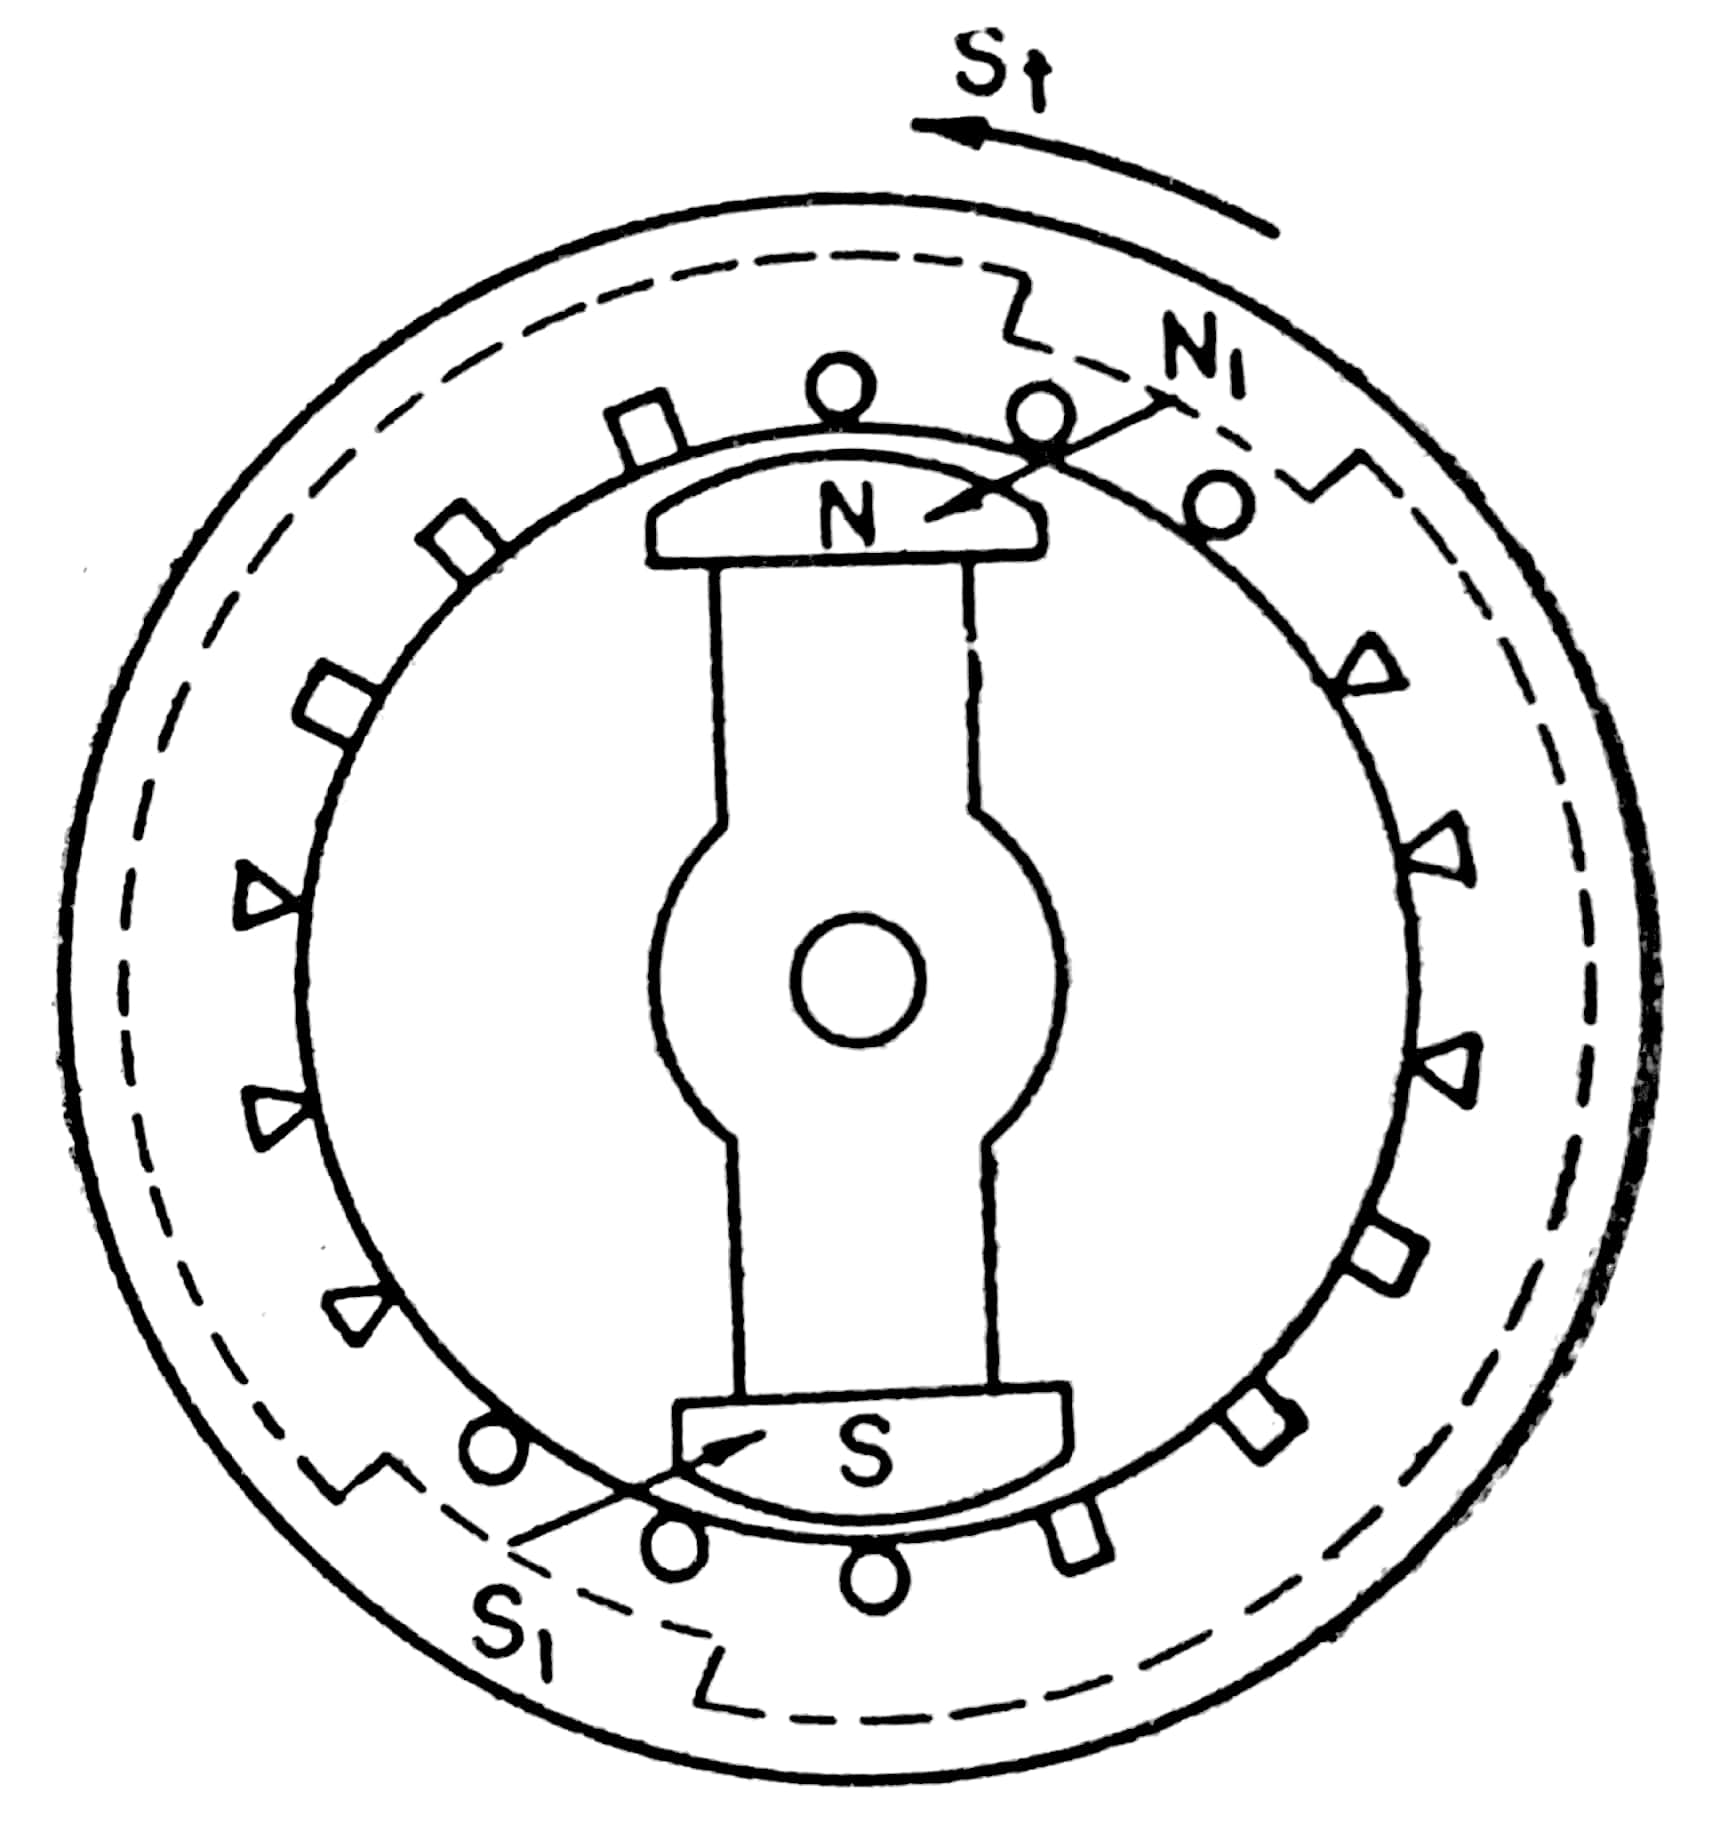
\includegraphics[scale=0.2]{imagens/20.png}
\caption{Máquina síncrona bipolar trifásica.}\label{fig:20}
\end{figure}

Quando o campo rotativo ultrapassa a posição da roda polar, esta última é solicitada a rodar em sentido contrário ao movimento $S_t$, destruindo assim o impulso anterior. O mesmo fenômeno repete-se a cada período e o conjugado médio resultante é constantemente igual a zero.

A roda polar poderá ser arrastada na rotação somente se for previamente portada a velocidade de sincronismo do campo rotativo, o qual deverá acioná-la deste momento em diante.

Logo que a roda alcança a velocidade de sincronismo, cria-se o campo rotativo no momento justo,a fim de que a roda polar e o campo rotativo se encontrem um com respeito ao outro na posição indicada na figura acima.

Do que foi exposto resulta que o motor síncrono não pode arrancar sozinho, devendo ser acionado previamente por meio de motor auxiliar. Este motor o faz alcançar a velocidade de sincronismo, a fim de poder executar o paralelo com a linha de alimentação.

Na fase de arranco, estando a máquina excitada, comporta-se como um alternador e, portanto, o interruptor só poderá ser fechado quando os aparelhos de  sincronismo indicam que isso é possível (exemplo de alternadores ligados em paralelo).

Depois de ter efetuado isso, pode-se suprimir a ação motora que serviu para executar o arranque. Nas fases estatóricas penetram as correntes que produzem o campo rotativo, mantendo a roda polar na rotação síncrona. A partir deste momento se inicia o funcionamento do motor síncrono.

Seja qual for a carga aplicada ao motor, a rotação do mesmo será invariável, dependendo esta da frequência de alimentação, sendo $$n = 60 * \frac{f}{p}$$.

Este tipo de motor funciona, ao variar a carga, com velocidade igual à do sincronismo, e por essa razão foi chamado de motor síncrono.

Dessa forma, o estudo do motor síncrono deve se iniciar no momento em que se efetua a manobra de paralelo com a linha de alimentação.

Neste momento a f.e.m que se gera em cada fase do induzido por efeito de rotação da roda polar contrapõe-se diretamente à tensão de linha de alimentação e o diagrama vetorial de cada fase se reduz aos dois vetores V e E iguais e sobrepostos, como na figura \ref{fig:21}.

\begin{figure}[ht!]
\center 
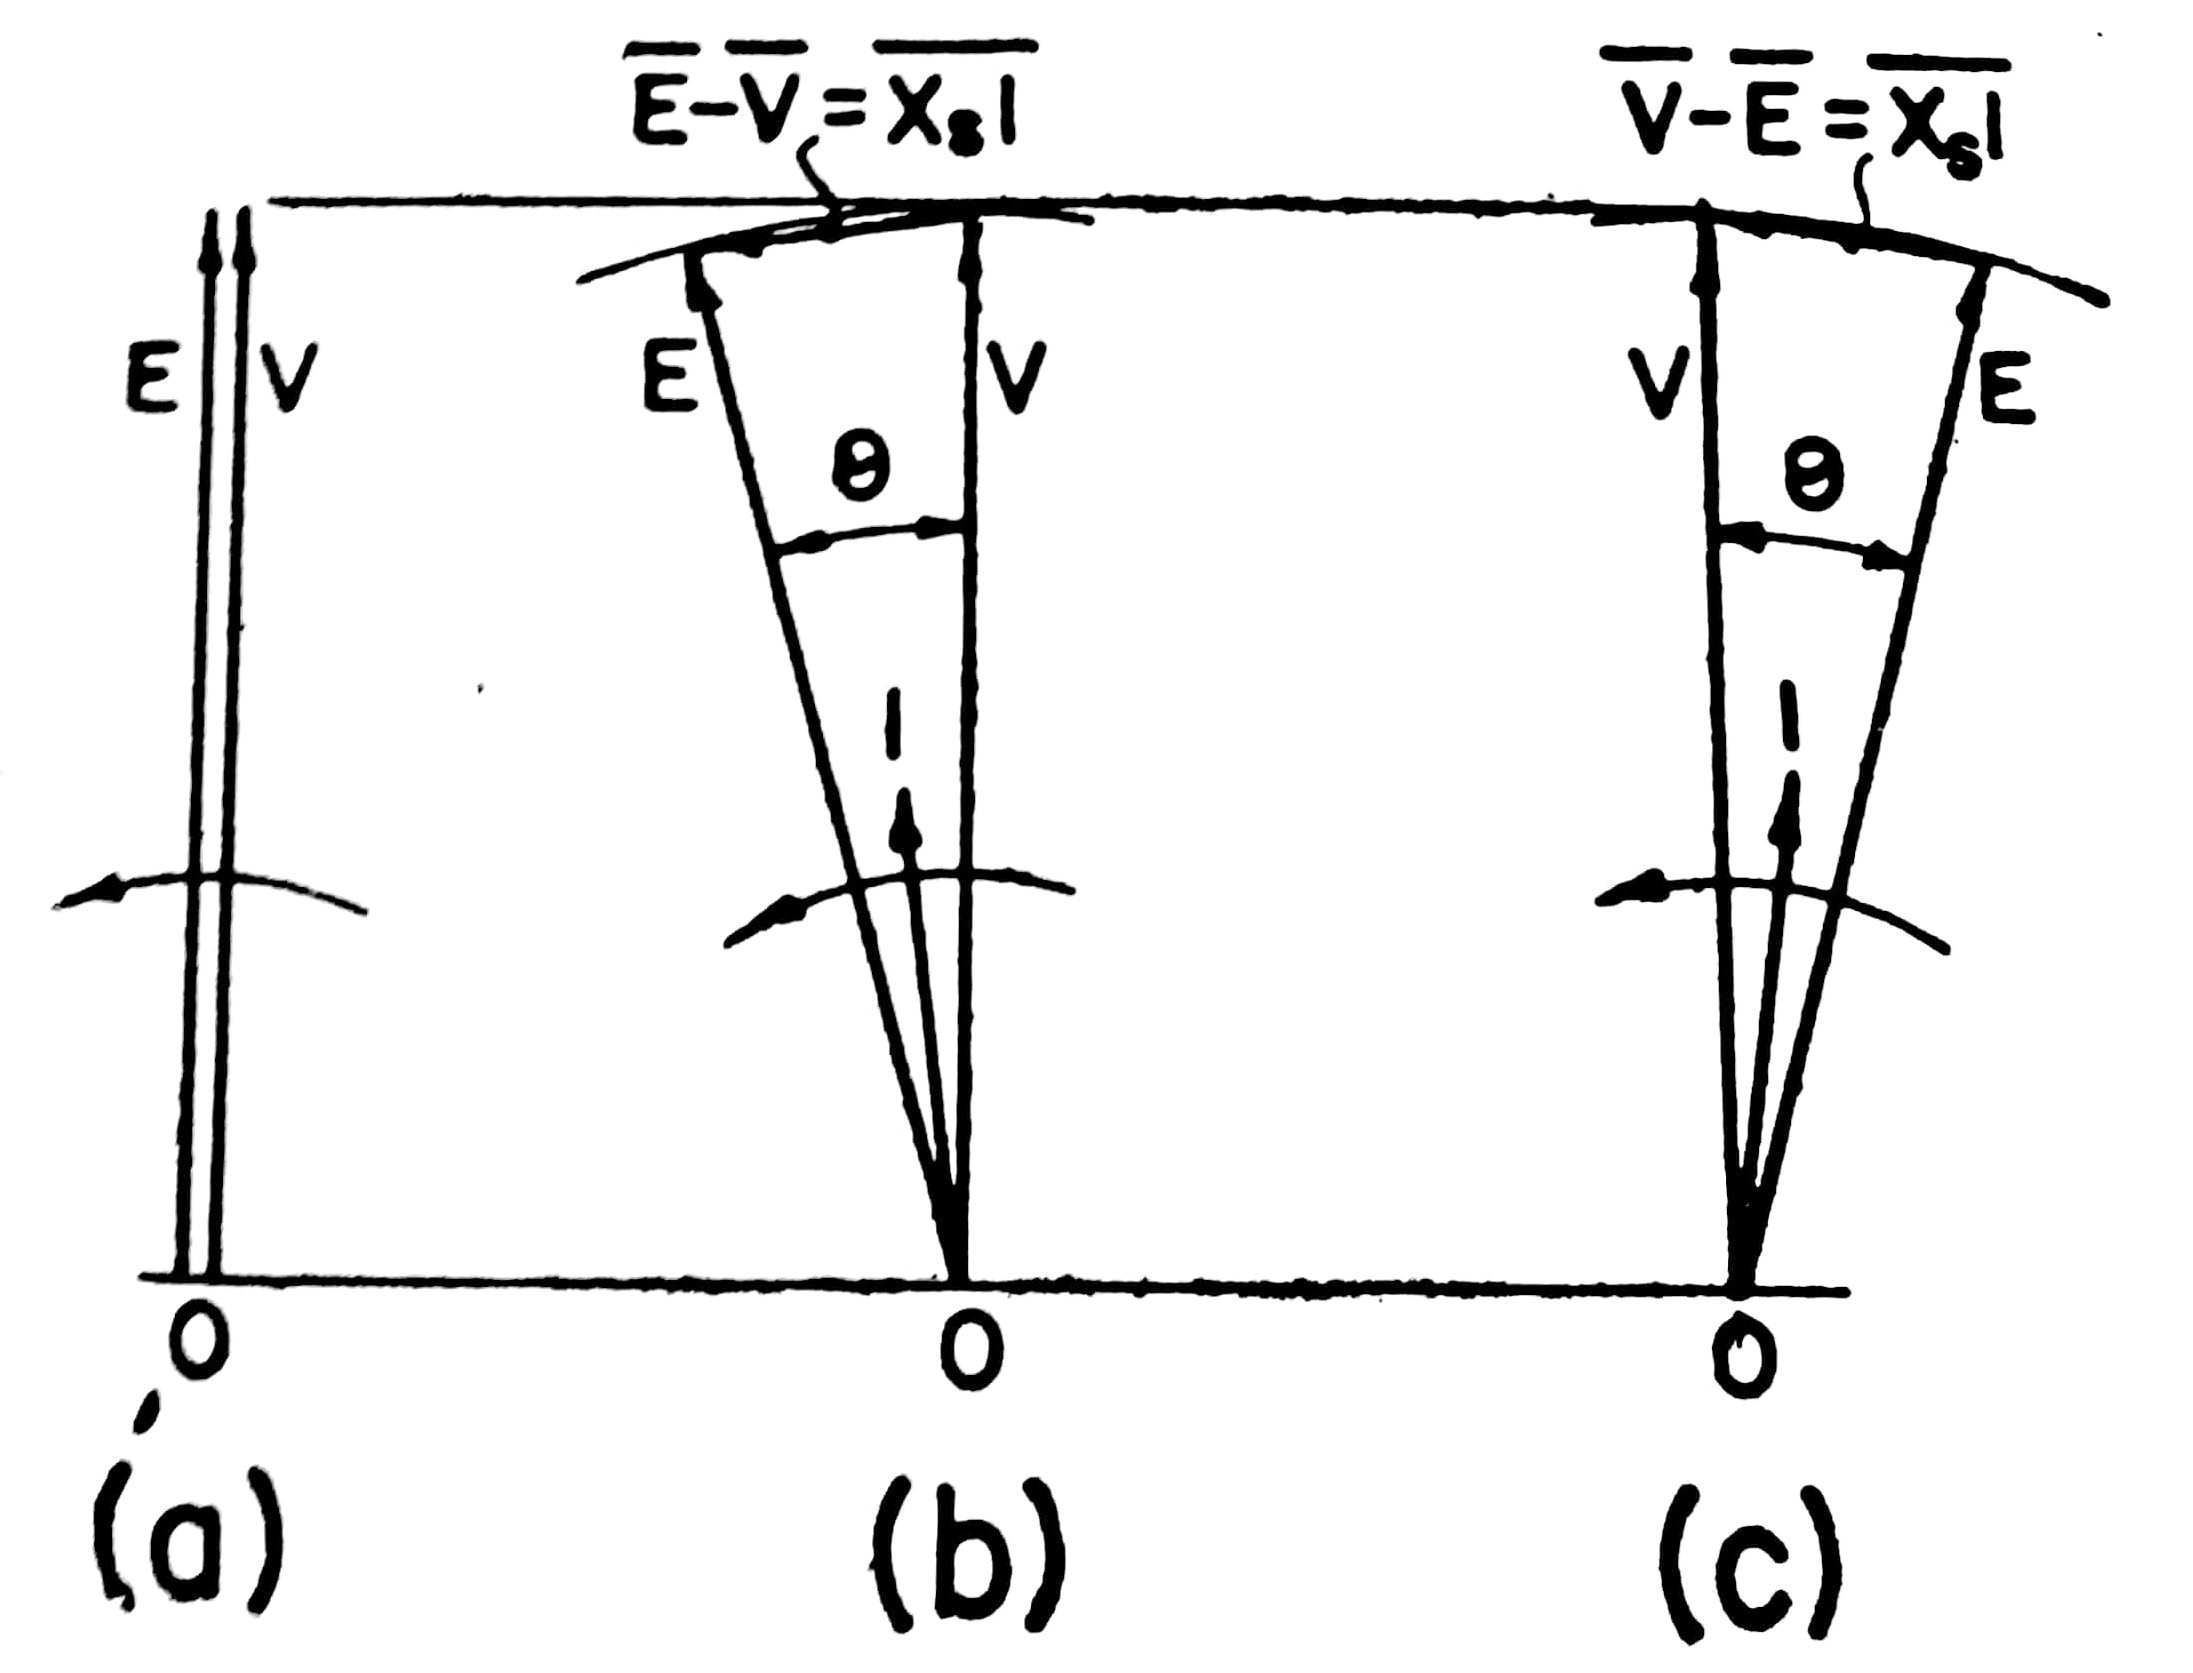
\includegraphics[scale=0.2]{imagens/21.png}\label{fig:21}
\caption{Diagrama vetorial sintético das fases do induzido.}
\end{figure}

Nessas condições, as fases do estator não fornecem nem absorvem corrente, pois existe o equilíbrio elétrico entre a f.e.m que se gera nas fases e a tensão que a estas é aplicada. A máquina funciona a vazio, mas para mantê-la nessas condições de funcionamento é necessário deixar ligado ao eixo o conjugado motor que serviu para arranque na manobra de paralelo, o que ainda é necessário para se compensarem todos os conjugados resistentes. A partir desse momento, aplicando-se ao eixo um conjugado motor, este imprimi à roda polar certo adiantamento, e a f.e.m sofre um adiantamento de fase com respeito à tensão de um ângulo $\theta$. Desse adiantamento origina-se o funcionamento da máquina como gerador, com base no diagrama vetorial já considerado na figura (b). Entre a f.e.m que se gera na fase da máquina e a tensão aplicada, determina-se a diferença vetorial ($\vec E$ - $\vec V$), que representa uma queda de tensão e obriga a máquina a fornecer a corrente capaz de provocar tal queda. Serão considerados somente os fenômenos de caráter indutivo, aos quais correspondem complexivamente a ação da reação do induzido e a do fluxo disperso. Tais fenômenos estão representados pela pela queda $X_s$ e $I$, devida à reatância síncrona $X_s$.

A corrente defasada de 90$^{\circ}$ em atraso, com respeito ao vetor ($\vec E$ - $\vec V$); é ,portanto, representada no diagrama da figura (b) pelo vetor $I$. Esta corrente resulta, assim, quase em fase com a f.e.m, e por isso, uma corrente fornecida essencialmente ativa. Tal corrente determina um conjugado resistente que estabelece o equilíbrio dinâmico com o conjugado motor que foi aplicado ao eixo da máquina para produzir o adiantamento $\theta$. A potência mecânica aplicada ao eixo, para vencer esse conjugado, se traduz em potência elétrica gerada e enviada para a linha.

Sobre o contrário, isto é, depois de ter executado o paralelo da máquina com a linha, aplicar sobre o eixo um conjugado freante em lugar de um motor. A roda polar sofre, então, certo atraso, e quando este se origina, a f.e.m também defasa em atraso de certo ângulo $\theta$, com respeito à tensão aplicada, e o diagrama da figura (a) transforma-se na figura (c). Entre a tensão aplicada $V$ e a f.e.m $E$, que no caso do motor atua como f.c.e.m, manifesta-se a diferença de potencial ($\vec V$ - $\vec E$). Nos enrolamentos da máquina circula, assim, em cada fase, uma corrente $I$ (não mais fornecida, mas absorvida) que, devendo estar a 90$^{\circ}$ em atraso com respeito ao vetor $\vec V$ - $\vec E$ = $\vec X_s$ $\vec I$, resulta na bissetriz do ângulo $\theta$.

Com a queda de tensão assim invertida, invertem-se também  as polaridades do campo rotativo. No funcionamento da máquina como gerador, o campo rotativo induzido provoca um conjugado freante. No funcionamento da máquina como motor, o rotativo provoca ações propulsoras.

No primeiro caso, a potência mecânica empregada para vencer o conjugado resistente corresponde à potência elétrica gerada e utilizada pela linha.

No segundo caso, o conjugado motor é representado pela potência mecânica gerada à custa da potência elétrica absorvida da linha.

O conjugado motor será maior, quanto maior for o ângulo $\theta$ de atraso entre a f.e.m com respeito à tensão. O resultado é que aumentando ou diminuindo a ação freante aplicada ao motor, isto é, aumentando-se ou diminuindo-se a carga que o motor deve vencer, aumenta ou diminui o ângulo $\theta$.

